% SC2001 — Chapter 2: Asymptotic Analysis
% No \documentclass — \included by modules/SC2001/main.tex (book class).
\chapter{Asymptotic Analysis}
\label{ch:asymptotics}

\begin{quote}
\emph{``We should forget about small efficiencies, say about 97\% of the time.''} --- Knuth. Asymptotic notation lets us forget the 97\% and compare the shape of growth itself.
\end{quote}

\noindent\textbf{Prerequisites:} Ch.~1 (RAM model, induction, sums/logs). This chapter formalises the $O(\cdot)$ language used in every later analysis.

\section*{Learning Outcomes}
After this chapter you will be able to:
\begin{enumerate}[label=(L\arabic*)]
    \item state the five asymptotic notations with quantifiers and negate them correctly;
    \item apply the limit method to classify functions;
    \item order the hierarchy $\log n \prec n \prec n\log n \prec n^{2}\prec 2^{n}$ and justify it;
    \item distinguish best-, worst-, and average-case analysis;
    \item write a recurrence for a recursive algorithm's running time (bridge to Ch.~3).
\end{enumerate}

% ============================================================
\section{Why Asymptotics?}
\label{sec:why-asymptotics}
RAM time is $T(n)=\sum (\text{cost}_{i}\times\text{count}_{i}(n))$, an unwieldy exact formula. Constants depend on compiler and hardware; what survives across machines is \emph{rate of growth}. Asymptotic notation suppresses constants and lower-order terms and compares $T(n)$ to a clean reference $g(n)$ for large $n$ only.

We consider functions $f,g:\mathbb{N}\to\mathbb{R}_{\ge 0}$ eventually non-negative. ``Large $n$'' is captured by $\exists n_{0}\,\forall n\ge n_{0}$.

% ============================================================
\section{The Five Notations}
\label{sec:five-notations}

\begin{definition}[$O$ --- asymptotic upper bound]
$f(n)=O(g(n))$ iff $\exists c>0\,\exists n_{0}\in\mathbb{N}\,\forall n\ge n_{0}:\;0\le f(n)\le c\,g(n)$.
\end{definition}

\begin{definition}[$\Omega$ --- asymptotic lower bound]
$f(n)=\Omega(g(n))$ iff $\exists c>0\,\exists n_{0}\,\forall n\ge n_{0}:\;0\le c\,g(n)\le f(n)$.
\end{definition}

\begin{definition}[$\Theta$ --- tight bound]
$f(n)=\Theta(g(n))$ iff $\exists c_{1},c_{2}>0\,\exists n_{0}\,\forall n\ge n_{0}:\;0\le c_{1}g(n)\le f(n)\le c_{2}g(n)$. Equivalently $f=O(g)$ and $f=\Omega(g)$.
\end{definition}

\begin{definition}[$o$ --- strict upper bound]
$f(n)=o(g(n))$ iff $\forall c>0\,\exists n_{0}\,\forall n\ge n_{0}:\;0\le f(n)<c\,g(n)$. That is, $f/g\to0$.
\end{definition}

\begin{definition}[$\omega$ --- strict lower bound]
$f(n)=\omega(g(n))$ iff $\forall c>0\,\exists n_{0}\,\forall n\ge n_{0}:\;0\le c\,g(n)<f(n)$. That is, $f/g\to\infty$.
\end{definition}

\begin{remark}[Quantifier order matters]
$O$ has $\exists c\,\exists n_{0}\,\forall n\ge n_{0}$; $o$ has $\forall c\,\exists n_{0}\,\forall n\ge n_{0}$. Negations swap quantifiers: $f\neq O(g)$ iff $\forall c>0\,\forall n_{0}\,\exists n\ge n_{0}: f(n)>c\,g(n)$. The abuse $f=O(g)$ means $f\in O(g)$ as a set.
\end{remark}

\begin{figure}[h]
\centering
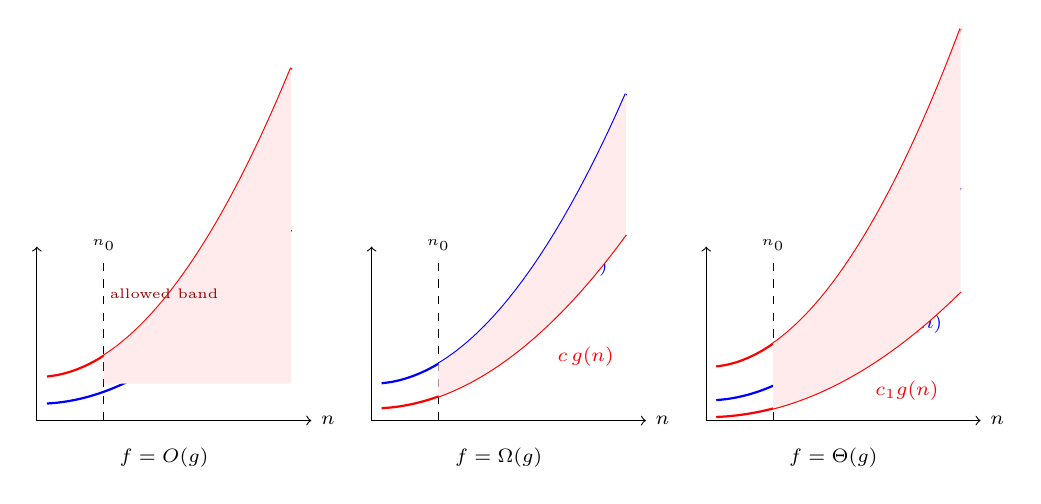
\begin{tikzpicture}[scale=0.85, every node/.style={font=\scriptsize}]
  % Axes shared style
  \def\h{2.2} \def\w{3.8}
  % --- O panel ---
  \begin{scope}
    \draw[->] (0,0) -- (\w+0.3,0) node[right] {$n$};
    \draw[->] (0,0) -- (0,\h+0.4) node[above] {};
    \draw[dashed] (1.0,0) -- (1.0,\h+0.2) node[above, font=\tiny] {$n_{0}$};
    \draw[blue, thick, domain=0.15:\w, smooth] plot (\x,{0.18*\x*\x+0.25});
    \node[blue] at (3.2,1.3) {$f(n)$};
    \draw[red, thick, domain=0.15:\w, smooth] plot (\x,{0.32*\x*\x+0.65});
    \node[red] at (3.2,2.35) {$c\,g(n)$};
    \fill[red!8] (1.0,0.55) -- plot[domain=1.0:\w] (\x,{0.32*\x*\x+0.65}) -- (\w,0.55) -- cycle;
    \node at (1.9,-0.55) {$f=O(g)$};
    \node[font=\tiny, red!60!black] at (1.9,1.9) {allowed band};
  \end{scope}
  % --- Omega panel ---
  \begin{scope}[xshift=5.0cm]
    \draw[->] (0,0) -- (\w+0.3,0) node[right] {$n$};
    \draw[->] (0,0) -- (0,\h+0.4) node[above] {};
    \draw[dashed] (1.0,0) -- (1.0,\h+0.2) node[above, font=\tiny] {$n_{0}$};
    \draw[blue, thick, domain=0.15:\w, smooth] plot (\x,{0.30*\x*\x+0.55});
    \node[blue] at (3.2,2.3) {$f(n)$};
    \draw[red, thick, domain=0.15:\w, smooth] plot (\x,{0.18*\x*\x+0.18});
    \node[red] at (3.2,0.95) {$c\,g(n)$};
    \fill[red!8] (1.0,0.50) -- plot[domain=1.0:\w] (\x,{0.18*\x*\x+0.18}) -- plot[domain=\w:1.0] (\x,{0.30*\x*\x+0.55}) -- cycle;
    \node at (1.9,-0.55) {$f=\Omega(g)$};
  \end{scope}
  % --- Theta panel ---
  \begin{scope}[xshift=10.0cm]
    \draw[->] (0,0) -- (\w+0.3,0) node[right] {$n$};
    \draw[->] (0,0) -- (0,\h+0.4) node[above] {};
    \draw[dashed] (1.0,0) -- (1.0,\h+0.2) node[above, font=\tiny] {$n_{0}$};
    \draw[red, thick, domain=0.15:\w, smooth] plot (\x,{0.35*\x*\x+0.80});
    \node[red] at (3.0,2.5) {$c_{2}g(n)$};
    \draw[blue, thick, domain=0.15:\w, smooth] plot (\x,{0.22*\x*\x+0.30});
    \node[blue] at (3.2,1.45) {$f(n)$};
    \draw[red, thick, domain=0.15:\w, smooth] plot (\x,{0.13*\x*\x+0.05});
    \node[red] at (3.0,0.45) {$c_{1}g(n)$};
    \fill[red!8] (1.0,0.22) -- plot[domain=1.0:\w] (\x,{0.13*\x*\x+0.05}) -- plot[domain=\w:1.0] (\x,{0.35*\x*\x+0.80}) -- cycle;
    \node at (1.9,-0.55) {$f=\Theta(g)$};
  \end{scope}
\end{tikzpicture}
\caption{$O$, $\Omega$, and $\Theta$ as eventually-sandwiching bands. Only behaviour for $n\ge n_{0}$ matters; constants $c,c_{1},c_{2}$ scale the reference $g(n)$.}
\label{fig:asymptotic-bands}
\end{figure}

Fig.~\ref{fig:asymptotic-bands} visualises the three bands. $o$ and $\omega$ require the sandwich to hold for \emph{every} $c>0$ (arbitrarily tight).

% ============================================================
\section{The Limit Method}
\label{sec:limit-method}
When limits exist, quantifier gymnastics reduces to calculus.

\begin{theorem}[Limit test]
Let $L=\lim_{n\to\infty}f(n)/g(n)$ (in $\mathbb{R}_{\ge0}\cup\{\infty\}$), assuming $g(n)>0$ eventually.
\begin{enumerate}[label=(\alph*)]
    \item If $0<L<\infty$ then $f=\Theta(g)$.
    \item If $L=0$ then $f=o(g)$ (hence $f=O(g)$).
    \item If $L=\infty$ then $f=\omega(g)$ (hence $f=\Omega(g)$).
\end{enumerate}
If $L$ does not exist (oscillation), the test is inconclusive and we return to definitions.
\end{theorem}

\begin{example}
$3n^{2}+5n+20=\Theta(n^{2})$ because $(3n^{2}+5n+20)/n^{2}\to3\in(0,\infty)$. Similarly $\log(n!)=\Theta(n\log n)$ since $n!\le n^{n}$ and $n!\ge(n/2)^{n/2}$, or via Stirling; we prove it rigorously in Ch.~3.
\end{example}

\begin{example}[Limits need care]
$f(n)=n^{1+\sin n}$ oscillates between $n^{0}$ and $n^{2}$; $f(n)/n$ has no limit and $f$ is neither $O(n)$ nor $\Omega(n^{2})$. Always check existence.
\end{example}

Useful rules: l'H\^opital for $\infty/\infty$, and $\log_{a}n=\Theta(\log_{b}n)$ for any $a,b>1$ (change of base is a constant factor). Hence we write simply $\Theta(\log n)$.

% ============================================================
\section{Growth Hierarchy}
\label{sec:hierarchy}

\begin{theorem}[Hierarchy]
For any $\epsilon>0$ and $c>1$:
\[
1 \prec \log n \prec n^{\epsilon} \prec n \prec n\log n \prec n^{1+\epsilon} \prec n^{2}\prec 2^{n}\prec n! \prec n^{n},
\]
where $a(n)\prec b(n)$ means $a(n)=o(b(n))$. In particular $\log n=o(n^{\epsilon})$, $n^{k}=o(c^{n})$ for any fixed $k$, and $c^{n}=o(n!)$.
\end{theorem}
\begin{proof}[Sketch]
Each claim is a limit: e.g.\ $\log n/n^{\epsilon}\to0$ by l'H\^opital, and $n^{k}/c^{n}\to0$ because exponentials dominate polynomials (apply l'H\^opital $k$ times). The rest is transitivity of $o$.
\end{proof}

\begin{figure}[h]
\centering
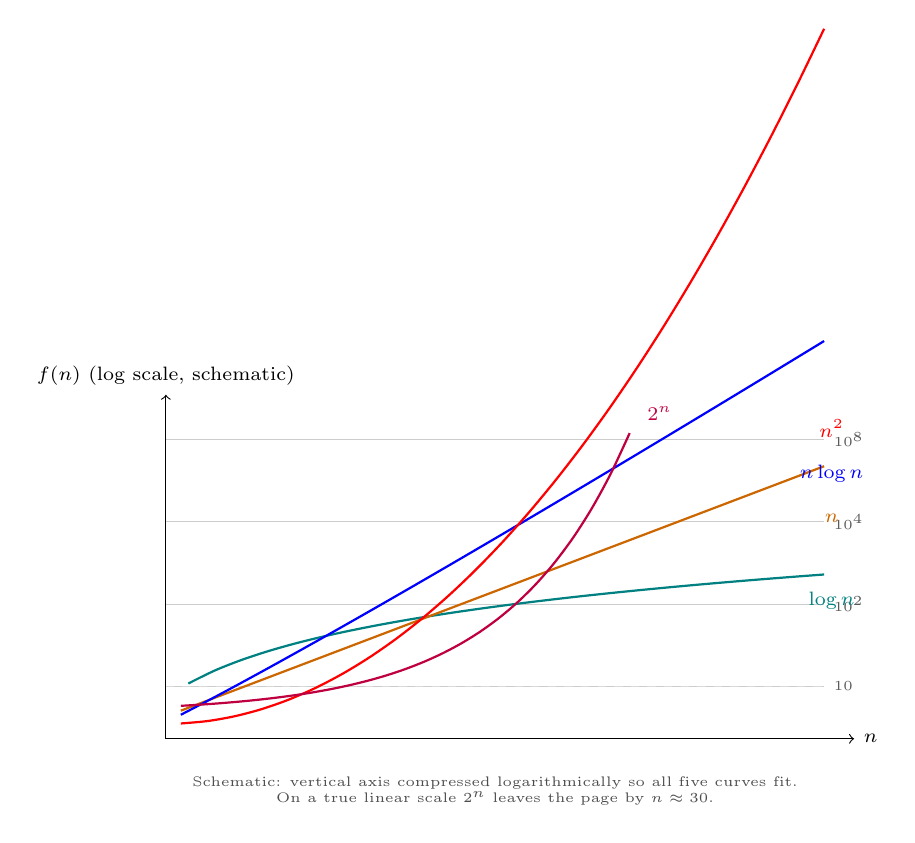
\begin{tikzpicture}[scale=0.95, every node/.style={font=\scriptsize}]
  \draw[->] (0,0) -- (9.2,0) node[right] {$n$};
  \draw[->] (0,0) -- (0,4.6) node[above] {$f(n)$ (log scale, schematic)};
  \foreach \y/\lbl in {0.7/10,1.8/10$^{2}$,2.9/10$^{4}$,4.0/10$^{8}$} \draw[gray!40] (0,\y) -- (8.8,\y) node[right, font=\tiny, gray!70!black] {\lbl};
  \draw[gray!30, dashed] (0,0.7) -- (8.8,0.7);
  \draw[teal, thick] plot[domain=0.3:8.8, smooth] (\x,{0.55+0.50*ln(\x+1)/ln(2)});
  \node[teal] at (8.9,1.85) {$\log n$};
  \draw[orange!80!black, thick] plot[domain=0.2:8.8, smooth] (\x,{0.30+0.38*\x});
  \node[orange!80!black] at (8.9,2.95) {$n$};
  \draw[blue, thick] plot[domain=0.2:8.8, smooth] (\x,{0.22+0.50*\x+0.08*\x*ln(\x+1)/ln(10)});
  \node[blue] at (8.9,3.55) {$n\log n$};
  \draw[red, thick] plot[domain=0.2:8.8, smooth] (\x,{0.20+0.12*\x*\x});
  \node[red] at (8.9,4.15) {$n^{2}$};
  \draw[purple, thick] plot[domain=0.2:6.2, smooth] (\x,{0.35+0.08*exp(0.62*\x)});
  \node[purple] at (6.6,4.35) {$2^{n}$};
  \node[font=\tiny, gray!60!black, align=center] at (4.4,-0.7) {Schematic: vertical axis compressed logarithmically so all five curves fit.\\On a true linear scale $2^{n}$ leaves the page by $n\approx30$.};
\end{tikzpicture}
\caption{Growth hierarchy on a logarithmically compressed vertical axis. Steeper eventually dominates: $\log n\ll n\ll n\log n\ll n^{2}\ll2^{n}$.}
\label{fig:growth-hierarchy}
\end{figure}

Fig.~\ref{fig:growth-hierarchy} shows the separation. Consequence: an $O(n\log n)$ sorting algorithm will beat an $O(n^{2})$ one for large $n$ no matter the constants --- the motivation for Ch.~4.

% ============================================================
\section{Best, Worst, and Average Case}
\label{sec:cases}
For input size $n$, let $T(I)$ be RAM steps on instance $I$ with $|I|=n$:
\begin{itemize}
    \item \textbf{Worst case:} $T_{\text{worst}}(n)=\max_{|I|=n}T(I)$ --- the guarantee.
    \item \textbf{Best case:} $T_{\text{best}}(n)=\min_{|I|=n}T(I)$ --- rarely used alone (overly optimistic).
    \item \textbf{Average case:} $T_{\text{avg}}(n)=\mathbb{E}_{I\sim D_{n}}[T(I)]$ under a distribution $D_{n}$ over size-$n$ inputs (often uniform). Requires specifying $D_{n}$.
\end{itemize}
When we say ``$\textsc{LinearSearch}$ is $O(n)$'' we mean $T_{\text{worst}}(n)=O(n)$; its best case is $\Theta(1)$ and its average case (uniform, key present) is $\Theta(n)$. \textsc{InsertionSort} is $\Theta(n)$ best case (already sorted, inner loop never runs) but $\Theta(n^{2})$ worst case.

Average-case analysis needs randomness: we fix $D_{n}$, then analyse $\mathbb{E}[T]$. Randomised algorithms (Ch.~8) instead randomise the \emph{algorithm} and bound $\mathbb{E}[T(I)]$ for every $I$.

% ============================================================
\section{Bridge to Recurrences}
\label{sec:recurrences-bridge}
Recursive algorithms do not have closed-form $T(n)$ directly; they satisfy \emph{recurrences}.

\begin{example}[Merge sort preview]
\textsc{MergeSort} on $n$ elements splits into two halves, recurses, then merges in $\Theta(n)$:
\[
T(n)=2\,T(n/2)+\Theta(n),\qquad T(1)=\Theta(1).
\]
Solving gives $T(n)=\Theta(n\log n)$ --- the canonical divide-and-conquer recurrence solved in Ch.~3.
\end{example}

In general a recurrence has form $T(n)=a\,T(n/b)+f(n)$ or $T(n)=T(n-1)+f(n)$ with base $T(n_{0})=c_{0}$. Ch.~3 develops three systematic solvers: substitution (guess-and-verify by induction), recursion trees (summing level costs), and the Master Theorem for $aT(n/b)+f(n)$. Asymptotics from this chapter is the language in which those solutions are stated.

% ============================================================
\section{Chapter Notes}
CLRS Ch.~3 is the standard reference for $O/\Theta/o/\omega$; Knuth (1976) introduced $O,\Omega,\Theta$ notation into CS. The limit method is an application of real analysis --- Rudin Ch.~3. Hierarchy facts follow from $\lim_{n\to\infty}(\log n)/n^{\epsilon}=0$, proved via l'H\^opital. Average-case analysis connects to probability (MH1813); we revisit it for QuickSort and hashing.

% ============================================================
\section{Exercises}
\label{sec:ch02-exercises}
\begin{enumerate}[label=E2.\arabic*, leftmargin=*, itemsep=0.7em]
    \item \textbf{Definitions and negations.} Let $f(n)=5n^{2}+3n$ and $g(n)=n^{2}$. (a) Prove $f=O(g)$ by exhibiting $c,n_{0}$. (b) Prove $f=\Omega(g)$. Conclude $f=\Theta(g)$. (c) Write the formal negation of ``$h(n)=o(g(n))$'' with quantifiers and use it to show $n^{2}\neq o(n^{2})$.

    \item \textbf{Limit method vs.\ oscillation.} Classify each pair using the limit method when applicable; otherwise return to definitions: (a) $f(n)=n\log n$, $g(n)=n^{1.5}$; (b) $f(n)=2^{n}$, $g(n)=3^{n}$; (c) $f(n)=n^{1+\sin n}$, $g(n)=n$. Determine which of $O,\Omega,\Theta,o,\omega$ hold (list all that apply).

    \item \textbf{Cases and distributions.} Consider \textsc{LinearSearch} for a key in $A[1\ldots n]$ (distinct elements, key present uniformly at random position). (a) Give $T_{\text{best}}(n)$, $T_{\text{worst}}(n)$ with $\Theta$ bounds. (b) Compute $T_{\text{avg}}(n)$ exactly as a sum and give its $\Theta$ class. (c) Suppose the key is absent with probability $1/2$ and otherwise uniform among positions. How does $T_{\text{avg}}(n)$ change?

    \item \textbf{Setting up recurrences.} Write recurrences (with base cases) for: (a) \textsc{RecursiveMax} that finds the maximum by comparing $A[n]$ with the max of $A[1\ldots n-1]$; (b) binary search on a sorted array of size $n$ (worst case); (c) Karatsuba-style: $T(n)=3T(n/2)+\Theta(n)$ --- do not solve, just explain in one sentence what $3$, $n/2$, and $\Theta(n)$ represent. Identify which cases from (a)--(c) fit the Master form $aT(n/b)+f(n)$.
\end{enumerate}
% End of Chapter 2
